\documentclass[10pt]{article}
\usepackage[spanish]{babel}
\usepackage{graphicx}
\usepackage[usenames,dvipsnames]{xcolor}
\usepackage{color}

%codigos: \begin{abstract} \end{abstract} es resumen
%nueva pagina \newpage
%colores predefinidos : white, black, red, green, blue, cyan, magenta, yellow
%\textcolor{blue}{text}
%\color{blue!20!black!30!green}{Prueba} mezcla de colores, conviene manejar solo 2 colores, es mas manejable



\begin{document}
{\centering
{\Large{Escuela Superior Polit\'ecnica del Litoral\\Facultad de Ingenier\'ia en Electricidad y Computaci\'on\\}}
\vspace{0.6in}

\includegraphics[scale=0.5]{espol.png}\\
\vspace{0.8in}
{\LARGE \textbf{\color{blue}{Lenguajes de Programaci\'on\\\vspace{0.3in}Experiencias de cada lenguaje}}\\
\vspace{0.5in}

%------------------------------------------------------------------------------------------%
\newpage
\tableofcontents

%------------------------------------------------------------------------------------------%
\newpage
\begin{flushleft}
\section{Github}
Es un repositorio en linea que usa un sistema de control de versiones.\\
Bastante agradable al usuario, porque permite compartir con otros los proyectos que se han subido.\\
\subsection{Conclusiones}
Es una herramienta muy \'util si es que trabajan algunas personas en el proyecto y si adem\'as el proyecto necesita ser mejorado o cambiado en el transcurso del tiempo.\\
\subsubsection{Experiencias Personales}
Me gust\'o mucho trabajar con github, porque es muy sencillo de utilizar, adem\'as que brinda un interesante sistema similar al de twitter en el cual hay gente siguiendo y gente a quien sigues.\\
Ha sido bastante bueno trabajar con Github, porque me sirvi\'o tambien en otra materia en la cual tuve que realizar un ensayo y lo tengo subido al Github.\\\vspace{0.1in}
Se que Github me servir\'a mucho en el futuro, tanto como repositorio como para mis futuros proyectos que requieran modificaciones, por eso mantengo con actividad la cuenta y la reviso peri\'odicamente.


%------------------------------------------------------------------------------------------%
\newpage
\section{\LaTeX{}}
Es un sistema de composici\'on de texto, orientado de manera especial a la creaci\'on de documentos y reportes cient\'ificos.
\subsection{Conclusiones}
Es bastante \'util para realizar algunas cosas que con un editor de texto se pudieran complicar.\\
Para alguien que nunca ha usado algo similar, puede llegar a ser molesto, pero con la pr\'actica se llega a acostumbrar y a mejorar en su manejo.
\subsubsection{Experiencias Personales}
Me ha parecido bastante agradable trabajar con \LaTeX{}, aunque al principio lo vi tan complicado.\\
Pude ver su utilidad porque en otra materia me pidieron desarrollar un trabajo con \LaTeX{}, mientras trabajaba en eso obtuve un poco mas de pr\'actica y ya se me hizo bastante f\'aci. No es una herramienta que usar\'ia siempre, pero si para ciertos casos, como por ejemplo, si necesitara el trabajo en pdf, no he visto que haya un modo mas f\'acil y efectivo que \LaTeX{}.

\end{flushleft}

%------------------------------------------------------------------------------------------%
\newpage
\begin{flushleft}
\section{Android}
\vspace{0.5in}
\begin{abstract}
\vspace{0.3in}
\large{Este es el primer trabajo de lenguajes de programaci\'on,para el cual las indicaciones fueron las de realizar un proyecto de aplicaci\'on m\'ovil, mas espec\'ifico en Android.\\
Hubieron algunas dificultades al principio, era algo nuevo para todos, a\'un no ten\'iamos clara la idea de lo que se har\'ia.\\
Entre algunas ideas, finalmente surgi\'o MY TWIN, algo que realmente nos pareci\'o novedoso y con alguna utilidad que se puede agregar a un dispositivo m\'ovil.\\
Se trabajo bastante con los recursos del tel\'efono y se hizo mucho \'enfasis en la proyecci\'on de tener un dispositivo con todo personalizado.}
\end{abstract}
\begin{center}
\vspace{0.3in}

\includegraphics[scale=0.5]{logo}\\
\vspace{0.3in}

\includegraphics[scale=0.2]{logAndroid}
\end{center}
\end{flushleft}

%------------------------------------------------------------------------------------------%
\newpage
\begin{flushleft}
\subsection{Introducci\'on}

\normalsize
MY TWIN una aplicaci\'on dirigida a toda clase de usuario mediante la cual podr\'as crear tu propio avatar, el cual se convertir\'a en tu asesor personal de tareas.

Una aplicaci\'on la cual jugar\'a con los estados de \'animo de tu avatar, los cuales estar\'an definidos por las diferentes tareas que cumplir\'a. Esto es que la aplicaci\'on no solo ser\'a para entretenimiento tendr\'a una funcionalidad que buscar\'a ayudar al usuario de una manera diferente, entretenida y personalizada.\\

\subsection{Idea}
\subsubsection{Problem\'atica}
Muchas veces tenemos nuestro celular o cualquier dispositivo m\'ovil en al cual podemos programar para que nos notifique o nos recuerde algunas tareas, pero eso es todo lo que hace.\\
Buscabamos entonces una funcionalidad extra al tel\'efono y que a la vez sea agradable al ususario.\\
Todo comenz\'o con una lluvia de ideas, donde algunas fueron muy simples y de poca utilidad y otrass en cambio eran muy complicadas y sin prestar el mayor benefecio, as\'i finalmente surgi\'o My Twin, idea que nos agrad\'o por que era posible de llevar a la realidad y adem\'as mejorar\'ia la funcionalidad de nuestro dispositivo m\'ovil.\\
My Twin como un entretenido gemelo virtual.\\
\vspace{0.3in}
\begin{center}
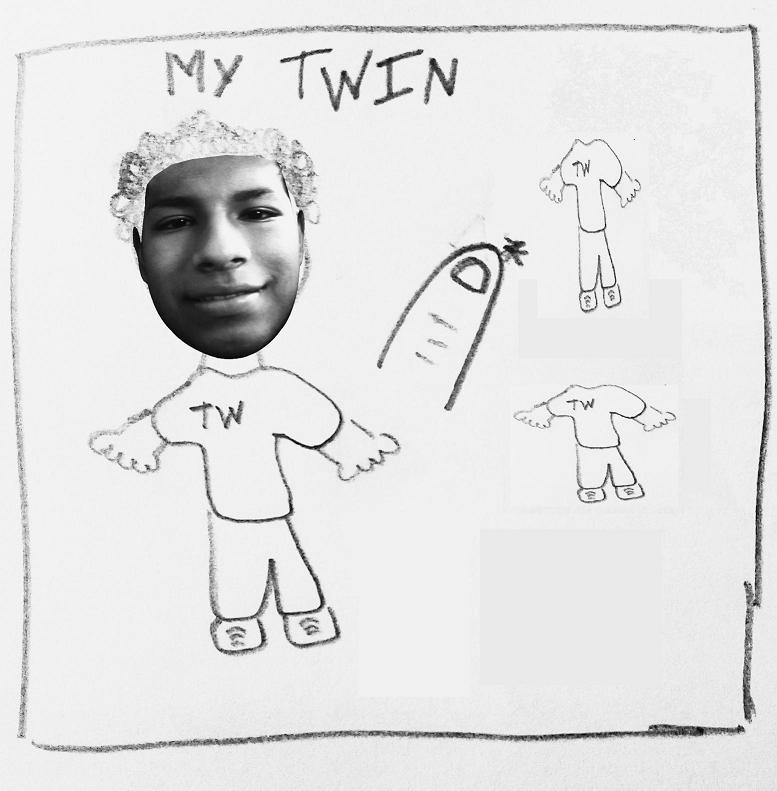
\includegraphics[scale=0.35]{bosquejoI1}
\end{center}

\end{flushleft}
}

%------------------------------------------------------------------------------------------%
\newpage
\begin{flushleft}
\subsubsection{Dise\~no}
El primer borrador fue trabajado en hojas con dibujos a mano, debido a que My Twin no era una sola pantalla est\'atica, sino que tiene algunas pantallas en la cual va cada una de las funciones.\\
Se dibujo algunos probables dise\~nos hasta llegar al que se tom\'o como modelo el siguiente.\\
\vspace{0.3in}
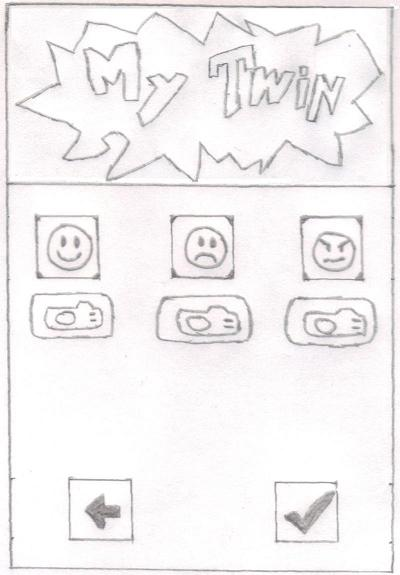
\includegraphics[scale=0.5]{Twin1}
\hspace{0.2in}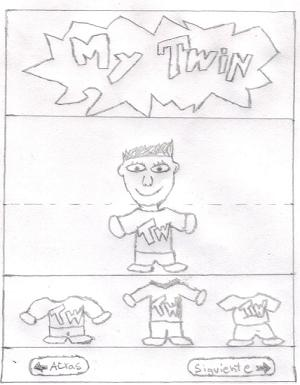
\includegraphics[scale=0.75]{Twin2}\vspace{0.2in}
\begin{center}
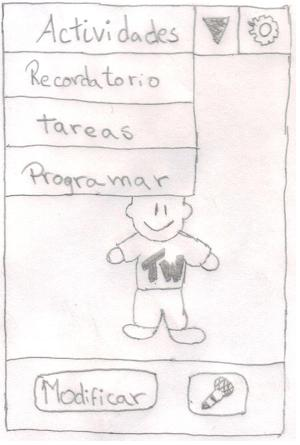
\includegraphics[scale=0.6]{Twin3}
\end{center}


\end{flushleft}


%------------------------------------------------------------------------------------------%
\newpage
\begin{flushleft}
\subsection{My Twin}
\subsubsection{Descripci\'on General}
\vspace{0.2in}
My Twin es una aplicaci\'on para dispositivo m\'ovil: \\\vspace{0.2in}\textbf{My Twin es divertido y original.\\
\vspace{0.1in}
\includegraphics[scale=0.6]{3.jpg}\\
\begin{center}
\vspace{0.1in}My Twin es realista.\\
\vspace{0.1in}
\includegraphics[scale=0.6]{droid.jpg}\\
\end{center}
\begin{flushright}
\vspace{0.1in}My Twin es amigable con el usuario.\\
\vspace{0.1in}
\includegraphics[scale=0.6]{amigableU.jpg}\\
\end{flushright}
}


\end{flushleft}

%------------------------------------------------------------------------------------------%
\newpage
\begin{flushleft}
\subsection{Funcionamiento (Manual de Usuario)}
\subsubsection{Pantalla Principal}

Pantalla Principal de My Twin, presionando en entrar, nos llevar\'a a la siguiente pantalla, si no tenemos aun creado el Twin, iremos a la pantalla de crear Twin, si ya lo tenemos, iremos directamente a la pantalla donde esta el menu y nuestro Twin.

\begin{center}
\vspace{0.1in}Pantalla Principal de inicio.\\
\vspace{0.1in}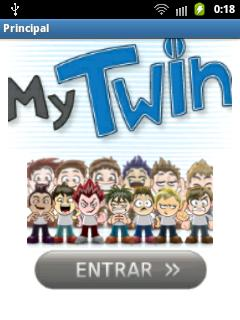
\includegraphics[scale=0.7]{PPrincipal}\\
\end{center}

\subsubsection{Creaci\'on de Twin}
Estas son las dos pantallas de creaci\'on del gemelo virtual, la primera es donde realizamos las fotos para la cara, d\'andole as\'i realismo; la segunda es para escoger un cuerpo, el cual le pone el lado original y divertido,donde todo es personalizable. \\
\begin{center}
\vspace{0.1in}
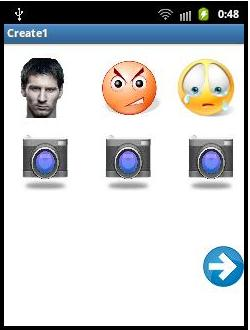
\includegraphics[scale=0.65]{create1.jpg}
\hspace{0.4in}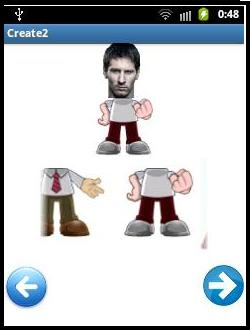
\includegraphics[scale=0.65]{create2.jpg}
\end{center}


%------------------------------------------------------------------------------------------%
\newpage
\subsubsection{Menu Tareas}
Luego de tener creado nuestro gemelo virtual, podemos ver el menu de tareas, el cual ser\'a la pantalla que veremos cada vez que entremos a la aplicaci\'on, el funcionamiento es sencillo, cuando vemos el menu se muestra en claras palabras lo que encontraremos al ingresar ah\'i.\\\vspace{0.2in}
\textbf{Tareas:} Nos llevar\'a a la pantalla de tareas, en la cual podremos programar los recordatorios de manera personalizada.\\\vspace{0.1in}
\textbf{Modificar:} Nos llevar\'a de regreso a la pantalla de creaci\'on de Twin, para que podamos realizar las modificaciones que queremos.\\\vspace{0.1in}
\textbf{Programar:} Nos permitir\'a programar el tel\'efono para casos especiales, como por ejemplo el ahorro de energ\'ia.\\

\begin{center}
\vspace{0.4in}
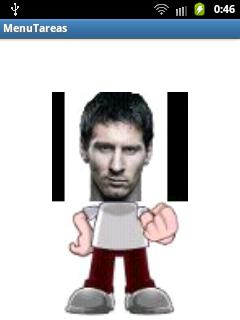
\includegraphics[scale=0.8]{MenuTareas1.jpg}
\hspace{0.4in}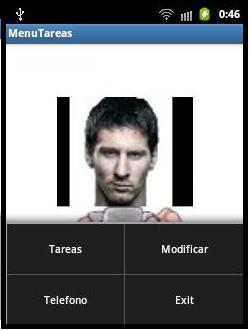
\includegraphics[scale=0.8]{MenuTareas2.jpg}
\end{center}

%------------------------------------------------------------------------------------------%
\newpage
\subsubsection{Nueva Tarea}
Aqu\'i podemos ver tres botones que hacen referencia al sonido, adem\'as de un reloj.\\
El funcionamiento es muy sencillo. En el reloj ponemos la hora que queremos establecer para recordar y los botones de grabacion funcionan así: uno para grabar, otro para detener y otro para reproducir la grabaci\'on.\\
Es importante recalcar que sin grabaci\'on no se puede avanzar, porque esto es parte del objetivo de buscar la originalidad, por esto es necesario que la tarea la recuerde con nuestra voz.\\
La otra parte importante es que podemos realizar tantas grabaciones como queramos, pues solo se escoger\'a la \'ultima, como parte de darle facilidad al ususario para que no tenga que iniciar el proceso nuevamente, esto se realiza de una manera sencilla en el mismo momento.\\

\begin{center}
\vspace{0.4in}
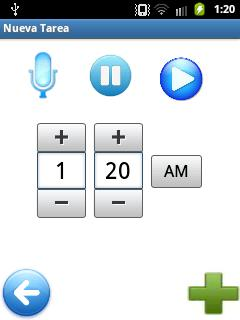
\includegraphics[scale=0.8]{NuevaTarea1.jpg}
\hspace{0.4in}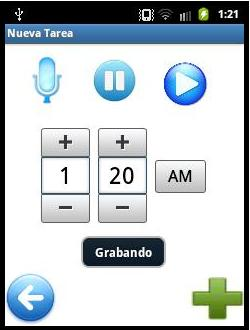
\includegraphics[scale=0.8]{NuevaTarea2.jpg}
\end{center}

%------------------------------------------------------------------------------------------%
\newpage
\subsubsection{Programar}
Esta funci\'on de la aplicaci\'on nos permite manejar recursos mas internos del dispositivo m\'ovil, de modo que se pueda programar su funcionamiento y manejarlo con un tiempo definido.\\

\begin{center}
\vspace{0.4in}
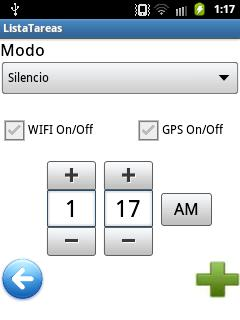
\includegraphics[scale=0.8]{Programar1.jpg}
\end{center}

%------------------------------------------------------------------------------------------%
\newpage
\subsection{Conclusiones}
Consideramos que logramos una aplicaci\'on completa que rompe la monoton\'ia de alarmas con tonos ruidosos
por una grabaci\'on de voz realizada por el usuario; aparte de eso la aplicaci\'on nos permite controlar los recursos 
b\'asicos del telefono.
\subsubsection{Experiencias Generales}
Realizar este trabajo no ha sido algo f\'acil, tuvimos varios inconvenientes. Al principio no encontrabamos la idea que nos ayudar\'ia a realizar este proyecto, luego vimos que este entorno de trabajo era diferente a lo que anteriormente hemos realizado, lo bueno es que contabamos con buenas bases de programaci\'on lo cual facilitaba un poco el entendimiento de lo nuevo que estabamos por ver.\\
En general el grupo siempre estuvo en contacto, de ese modo siempre se avanzaba en el trabajo, algunas veces tuvimos que trabajar hasta muy tarde por la noche, pero, a\'un as\'i vali\'o la pena, porque el trabajo se present\'o completo cumpliendo las expectativas que ten\'iamos acerca de la aplicaci\'on, adem\'as que ayud\'o a unir al grupo en amistad, pues cada problema que se presentaba se resolv\'ia realizando una reuni\'on ya sea f\'isicamente o por medio del internet.\\
Muchas de las cosas hubo que investigarlas puesto que esta era una experiencia nueva para todos y ninguno ten\'ia el conocimiento de lo que realizar\'iamos. Para resolver de manera mas eficiente, cada uno investigaba una parte y luego en reuni\'on expresabamos lo que hab\'iamos encontrado; en conjunto aprendimos cada uno de la experiencia del otro y de la informaci\'on que le toco buscar.\\
El entorno de trabajo para Android fue un poco complicado, pero sirvi\'o para darnos un empuje a lo que ser\'ian los otros proyectos de la materia, pudimos ver desde otra perspectiva la programaci\'on utilizando otras herramientas para trabajar; el hecho de tener exposiciones peri\'odicas del avance del proyecto nos presionaba precisamente a eso, que el proyecto estuviese en marcha, de este modo no nos atrasamos ni en terminar el trabajo ni en presentarlo.\\
\vspace{0.1in}Finalmente toda experiencia es y ha sido enriquecedora desde el punto de vista de conocimiento.
\subsubsection{Experiencias Personales}
\textbf{Kevin Marlon Calder\'on Barrera.- } En general se puede hablar de una muy buena experiencia, algo diferente a los dem\'as proyectos de programaci\'on que he tenido, pero que se pudo realizar y dej\'o una gran satisfacci\'on luego de ver el resultado del trabajo.\\\vspace{0.1in}
Debo reconocer que el trabajo en equipo y los buenos tutoriales existentes en internet ayudaron a que se pueda realizar este proyecto, porque era un poco extenso para hacerlo solo, adem\'as que se trataba de algo nuevo.\\
Entre las cosas que me gustaron de este trabajo es que la l\'ogica era similar a la que aprendimos en la materia de programaci\'on orientada a objetos, adem\'as que tratabamos algo nuevo que no se hab\'ia hecho, algo que nos hac\'ia diferente a los que ya se han dado de la materia y de paso los primeros.\\\vspace{0.1in}
Por otro lado algo que no me gusto de ese entorno es que muchas veces se presentaban errores y no entend\'ia a que se deb\'ian, tambi\'en era algo complicado de trabajar porque solo dispon\'iamos de un dispositivo m\'ovil y lo que funcionaba en el computador no daba el mismo resultado en el dispositivo, esto obligo a que siempre que trabajemos tengamos que estar todos conectados a internet y a trabajar de manera sincronizada.

%------------------------------------------------------------------------------------------%
\newpage
\section{Python}
\vspace{0.4in}
\begin{abstract}
\vspace{0.2in}
\large{Este es el segunto trabajo de Lenguajes de Programaci\'on, donde se nos pidi\'o realizar un proyecto en Python el cual utilizara sonidos para hallar la salida o las posibles respuestas, m\'as espec\'ifico, se nos pidi\'o realizar un juego que tenga como recurso principal los sonidos.\\
El tema de proyecto escogido fue elementsBalls, el cual b\'asicamente es un juego que exige desarrollar la agilidad mental, porque da una respuesta y se tiene que hallar la salida en el menor tiempo posible.\\
elementsBalls ha sido desarrollado totalmente en python utilizando la librer\'ia pygame. Python es bastante estable y da mucha flexibilidad al momento de programar, esto hizo de esta experiencia algo bastante agradable.\\
Con todo esto elementsBalls es un juego bastante interesante, con interacci\'on entre el jugador y el juego, es un juego que te desaf\'ia a desafiarte.}
\end{abstract}
\begin{center}
\vspace{0.3in}
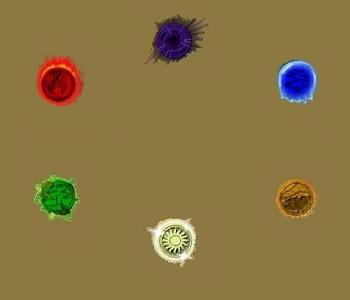
\includegraphics[scale=0.5]{gameEnd}
\\\vspace{0.3in}

\includegraphics[scale=0.2]{logPython}\\python
\end{center}


%------------------------------------------------------------------------------------------%
\newpage
\begin{flushleft}
\subsection{Introducci\'on}

\normalsize
elementsBalls es una aplicaci\'on de tipo juego para computadora, el cual propone algo diferente al usuario, un juego sencillo pero con las caracteristicas necesarias para convertirse en un juego completo al punto de convertirse en un favorito para el usuario.\\
Los componentes que tiene son:\\
\begin{itemize}
\item{}\textbf{Idea original}, la cual surgi\'o luego de un largo tiempo de pensar y dar vueltas en torno a los requerimientos del proyecto.
\item{}\textbf{Sencillo de entender}, porque el juego en realidad es tan sencillo, solo una pelota que debe llegar a una meta.
\item{}\textbf{Con diversas opciones}, esto evita la monoton\'ia, porque el nombre del juego es elements, que esta en plural, con esto nos indica que no solo ser\'a una pelota comun y corriente la que llegar\'a a la meta.
\item{}\textbf{Es un reto}, debido a que tenemos un tiempo l\'imite para completar la mayor cantidad de niveles.
\item{}\textbf{Permite la competencia}, podemos comparar y competir con nuestros amigos, desafiandonos a superar la cantidad de niveles de ellos en el mismo tiempo.
\end{itemize}

\end{flushleft}

%------------------------------------------------------------------------------------------%
\newpage
\subsection{Manual del Juego}
En esta seccion no hay mucho de que hablar, porque es bastante sencillo de entender, pero se expondr\'a de la forma mas amplia acerca del juego.\\
\begin{center}
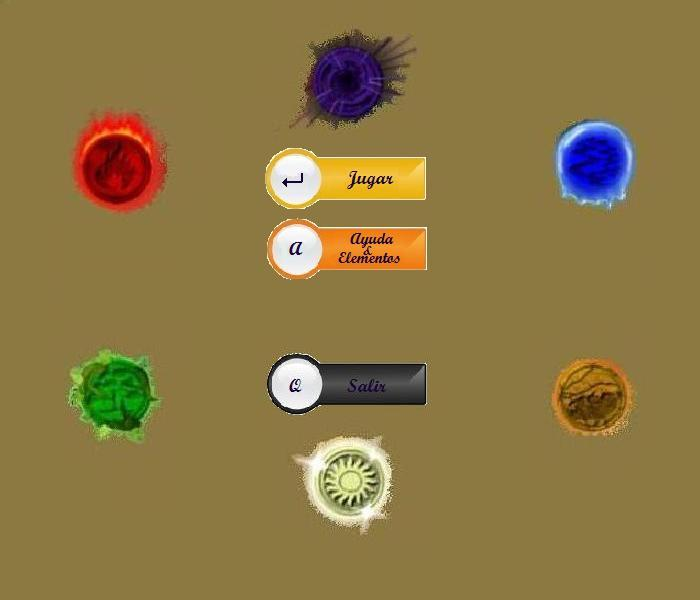
\includegraphics[scale=0.7]{newMain}
\end{center}
La primera vez que entramos escuchamos la grabaci\'on que nos indica como entrar a las tres opciones de la pantalla inicial, aunque tampoco es d\'ificil de entender porque tambi\'en se muestra gr\'aficamente
\vspace{0.3in}
\begin{itemize}
\item{}Presionando ``enter" pasaremos a \textbf{Jugar}, esto es un juego nuevo.
\item{}Presionando ``a"\ iremos a un menu que nos indicar\'a la \textbf{Ayuda y Elementos}.
\item{}Presionando ``q" vamos a \textbf{Salir} del juego.
\end{itemize}

%------------------------------------------------------------------------------------------%
\newpage
\subsubsection{Jugar}
La siguiente imagen muestra una probable forma de uno de los niveles al empezar un juego, la raz\'on por la cual es probable es porque no se va a dar el caso de que se vean iguales, porque la generaci\'on de los obst\'aculos y del tama\~no y tipo de obst\'aculo es totalmente aleatorio.\\
Se puede observar en la parte baja una pelota, en este caso del tipo fuego y obst\'aculos rectangulares de diversos tipos, mientras que al principio del nivel escuchamos la pista que nos da para avanzar al siguiente nivel, que en este caso fue ``Izquierda"\ esto quiere decir que la salida estar\'a a la izquierda.
\begin{center}
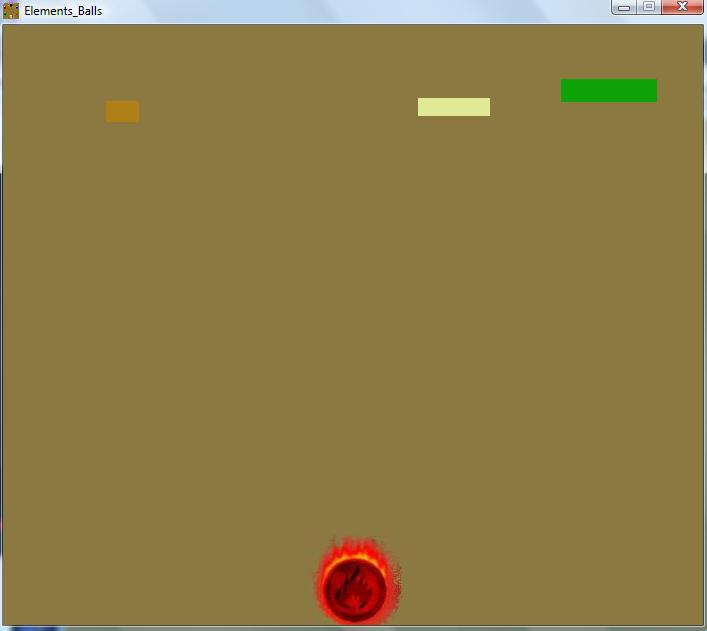
\includegraphics[scale=0.6]{jugar1}
\end{center}
\vspace{0.2in}Con las direccionales ubicamos la pelota hacia la izquierda y con la barra espaciadora la lanzamos.\\
Algo que nos puede ser \'util es conocer que podemos darle direcci\'on a la pelota, esto se logra con las direccionales, con la de arriba la pelota tendr\'a cierta inclinaci\'on hacia la derecha, mientras que con la de abajo se dar\'a hacia la izquierda.5

%------------------------------------------------------------------------------------------%
\newpage
Finalmente como vemos en la figura, la pelota ha sido lanzada, ha cambiado un poco su color porque hizo uso de su efecto, con el cual quem\'o el obst\'aculo para poder pasar, pero se apag\'o el fuego, eso quiere decir que us\'o su efecto.\\
Si no se lleg\'o a la meta al primer intento se puede volver a intentar, con lo \'unico presente que se ha consumido algo del tiempo, la pelota al salir estar\'a como nueva, con sus efectos sin utilizar.
\begin{center}
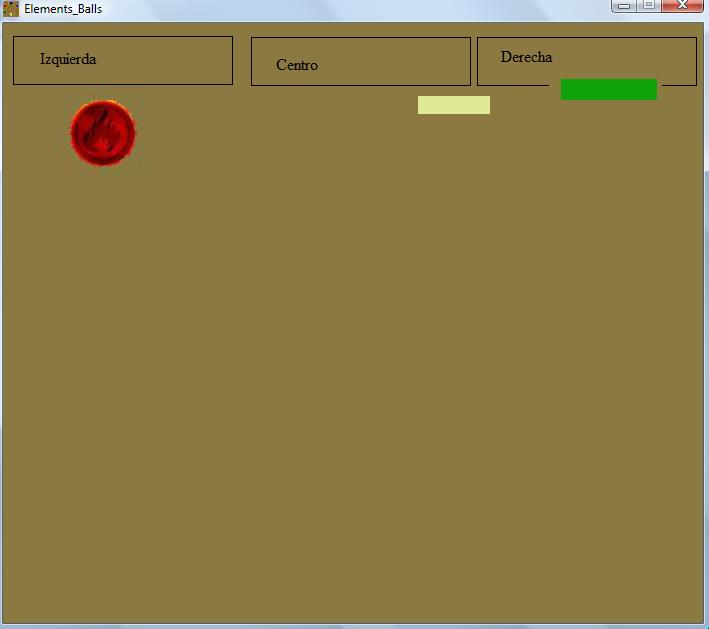
\includegraphics[scale=0.4]{jugar2}
\end{center}

A la imagen se le agreg\'o la meta, para que se pueda visualizar que se est\'a llegando y a donde se deber\'ia llegar.\\\vspace{0.1in}
\textbf{Juego Finalizado}\\
Al terminar el tiempo se ve una pantalla que nos indica hasta que nivel hemos llegado en un minuto que es el tiempo l\'imite que da el juego.
\begin{center}
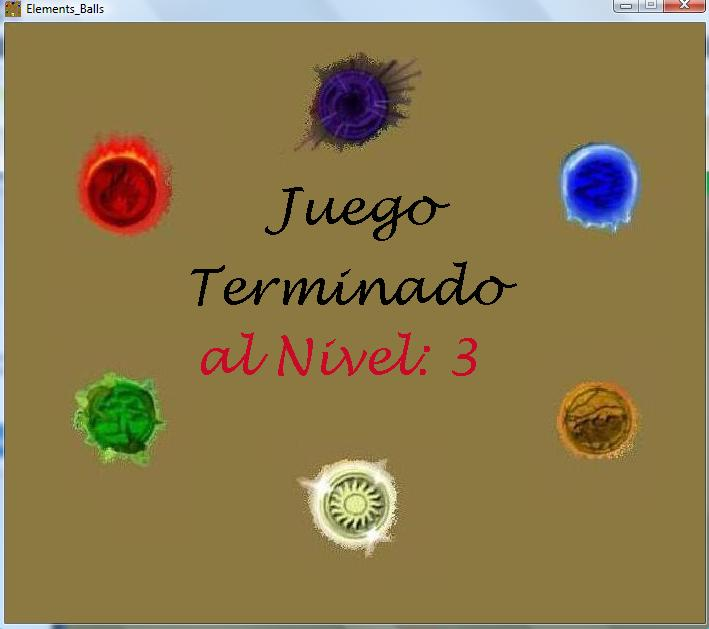
\includegraphics[scale=0.4]{jugar3}
\end{center}

%------------------------------------------------------------------------------------------%
\newpage
\subsubsection{Ayuda y Elementos}
Al principio escuchamos la grabaci\'on que nos dice el objetivo del juego.\\
En la imagen veremos las diferentes imagenes que representan a una pelota con un elemento diferente y as\'i mismo una letra que la identifica, casualmente estas letras est\'an todas juntas y esto es porque as\'i como en la ayuda podemos escucharla con ese tecla, en el juego la llamamos para utilizarla con las mismas teclas.
\begin{center}
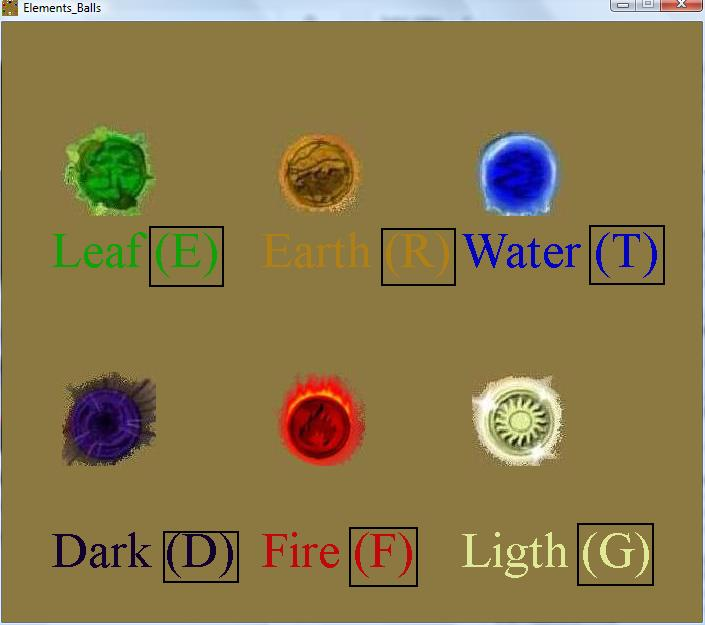
\includegraphics[scale=0.7]{ayudaEle}
\end{center}

%------------------------------------------------------------------------------------------%
\newpage
Ahora esto es lo que hace cada elemento junto est\'a la letra con la cual es llamado.\\
Aquellos obst\'aculos que no se ven nombrados, quiere decir que seguir\'an siendo obst\'aculos para ese elemento y har\'an rebotar a la pelota.
\begin{itemize}
\item{}\textbf{D-Dark:} Pasa sin problemas los obst\'aculos de su mismo tipo y los de tipo agua, destruye los de tipo tierra.
\item{}\textbf{F-Fire:} Pasa sin problemas los obst\'aculos de su mismo tipo, su fuego le permite atravesar cualquier otro tipo de obst\'aculo y queda apagado perdiendo su fuego. Si el obst\'aculo al que se encuentra fuese de agua, el fuego se apagar\'a y adem\'as rebotar\'a.
\item{}\textbf{G-Ligth:} Pasa sin problemas los obst\'aculos de su mismo tipo y los de tipo fuego, elimina los obst\'aculos de tipo planta.
\item{}\textbf{E-Leaf:} Pasa sin problemas los obst\'aculos de su mismo tipo y los de tipo oscuridad, puede eliminar los obst\'aculos de tipo planta, la desventaja que tiene es que es ligeramente mas lento.
\item{}\textbf{R-Earth:} Pasa sin problemas los obst\'aculos de su mismo tipo, de hecho puede destruir cualquier obst\'aculo con la excepci\'on de los de tipo luz, porque la tierra es un elemento que pertenece a su dominio. Tiene la desventaja de ser bastante lento, el m\'as lento de los elementos.
\item{}\textbf{T-Water:} Pasa sin problemas los obst\'aculos de su mismo tipo adem\'as de ``apagar" los del tipo fuego. Es el mas veloz de los elementos.
\end{itemize}
\end{flushleft}

%------------------------------------------------------------------------------------------%
\newpage
\begin{flushleft}
\subsubsection{Salir}
\begin{center}
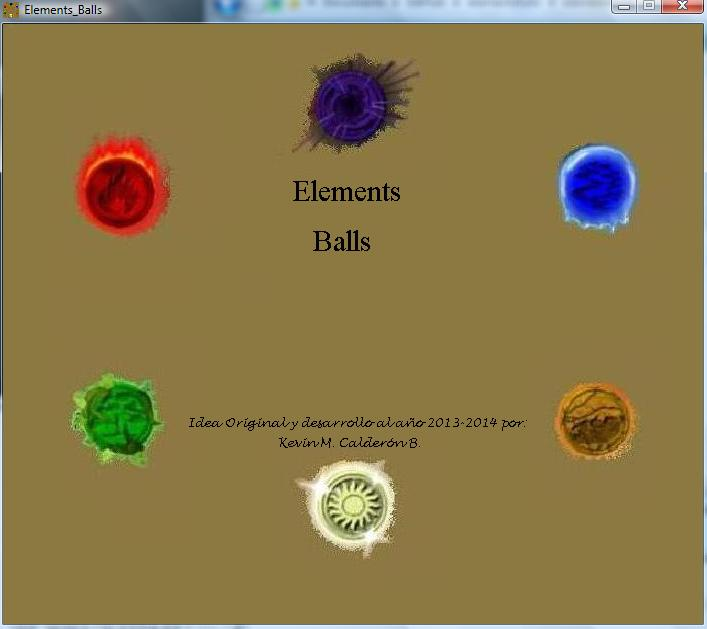
\includegraphics[scale=0.7]{salir1}
\end{center}
Esta es la pantalla que vemos al presionar ``q"\ o al dar clic en la ``x" de salir que tiene la ventana.\\
En esta pantalla vemos el nombre del juego y algo similar a cr\'editos, porque indican el nombre del desarrollador y el a\~no de cuando fue desarrollado.

%------------------------------------------------------------------------------------------%
\newpage
\subsection{Estado Actual}
En el link de github que se muestra a continuacion:\\\vspace{0.1in}\hspace{0.5in}https://github.com/kevmacal/elementsBalls.git\\\vspace{0.1in}
Encontraremos un documento de texto que nos dice el estado actual del juego, las modificaciones que se dar\'an en un futuro, adem\'as de las que ya se han dado.\\
Tambi\'en encontraremos la versi\'on liberada actual del juego. Para este d\'ia solamente se tiene como versi\'on liberada un demo que es el ejecutable del juego, pero una versi\'on que a\'un est\'a pasando pruebas hasta que llegue a ser mejorada y poder liberar una primera versi\'on.\\\vspace{0.1in}
Novedades: Documento que especificar\'a las novedades de la versi\'on actual y as\'i mismo permitir\'a conocer los futuros planes
para el mejoramiento del juego elements Balls.

%------------------------------------------------------------------------------------------%
\newpage
\subsection{Conclusiones}
Se ha llegado a un buen trabajo, un juego que tiene muchas buenas cualidades y que puede ser mejorado. Este trabajo esta en esa misma etapa, el lenguaje que se ha utilizado hizo posible que se complete hasta el estado que esta, pero se puede mejorar con el mismo lenguaje.\\
Este proyecto fue realizado en su totalidad por un solo desarrollador, por lo tanto las experiencias generales que se dar\'a una visi\'on general del lenguaje, para dejar algo mas espec\'ifico que ser\'ia descrita en las experiencias personales.
\subsubsection{Experiencias Generales}
Al igual que todo trabajo en este se tuvo que realizar un duro trabajo de investigaci\'on, previo al momento de programar, porque el esquema era orientado a objetos, que es algo que si exist\'ia el conocimiento previo, pero el lenguaje era algo totalmente nuevo.\\
El trabajo se llego a hacer un poco largo, porque al principio resultaba complicado, por esta raz\'on pasaba el tiempo sin mucho progreso.
Algo bastante bueno de python es que es muy sencillo de entender, por este motivo una vez que se pod\'ia entender hacia donde se quer\'ia llegar y se comprend\'ia como era la programaci\'on en python, el trabajo se hizo mas ligero y entretenido.\\

\subsubsection{Experiencias Personales}
Personalmente puedo decir que trabajar en Python ha sido una grata experiencia, ha sido algo bastante bueno aprender algo nuevo y pude notar que python es un lenguaje bastante bueno porque me daba bastante flexibilidad, facilitaba mucho el poder declarar las variables sin tener que especificar de que tipo era, solamente ten\'ia que ponerle un nombre bastante l\'ogico y que facilmente se asocie a lo que representaba y as\'i de f\'acil ya estaba lista la variable para usarse.\\\vspace{0.1in}
Entre lo que me gust\'o de python se puede resaltar la facilidad que presta pygame para llamar sonidos, poner a reproducir un sonido era tan sencillo, era como poner ``play" por un lado y para detenerlo ``stop" por otro. El manejo de eventos de python lo ten\'ia en una lista, se la recorr\'ia y as\'i facilmente pod\'ia encontrar lo que  iba haciendo con el teclado, como por ejemplo que tecla hab\'ia sido presionada.\\\vspace{0.1in}
Pero no me gustaba que cuando ten\'ia alg\'un error solo se ca\'ia el programa cuando en la ejecuci\'on entrabamos al error, de modo que si exisit\'ia alg\'un error en una parte que no se entraba mucho, tomar\'ia mucho tiempo en que sea descubierto. En cuanto a error me refiero a errores que se dieron en pruebas; en el momento de trabajar en el proyecto no pas\'e por eso, pero, eso me hizo demorar m\'as en las pruebas.

%------------------------------------------------------------------------------------------%
\newpage
\section{Haskell}
\vspace{0.4in}
\begin{abstract}
\vspace{0.2in}
\large{Tercer trabajo de programaci\'on, en el cual se nos ped\'ia utilizar el lenguaje funcional de Haskell para resolver el juego de mastermind en menos de 12 pasos.\\
Durante la ejecuci\'on se deb\'ia de poder mostrar el puntaje en cuanto a colores acertados y posiciones acertadas.\\
El proyecto no pudo ser terminado en el plazo establecido.\\}
\end{abstract}
\begin{center}
\vspace{0.3in}
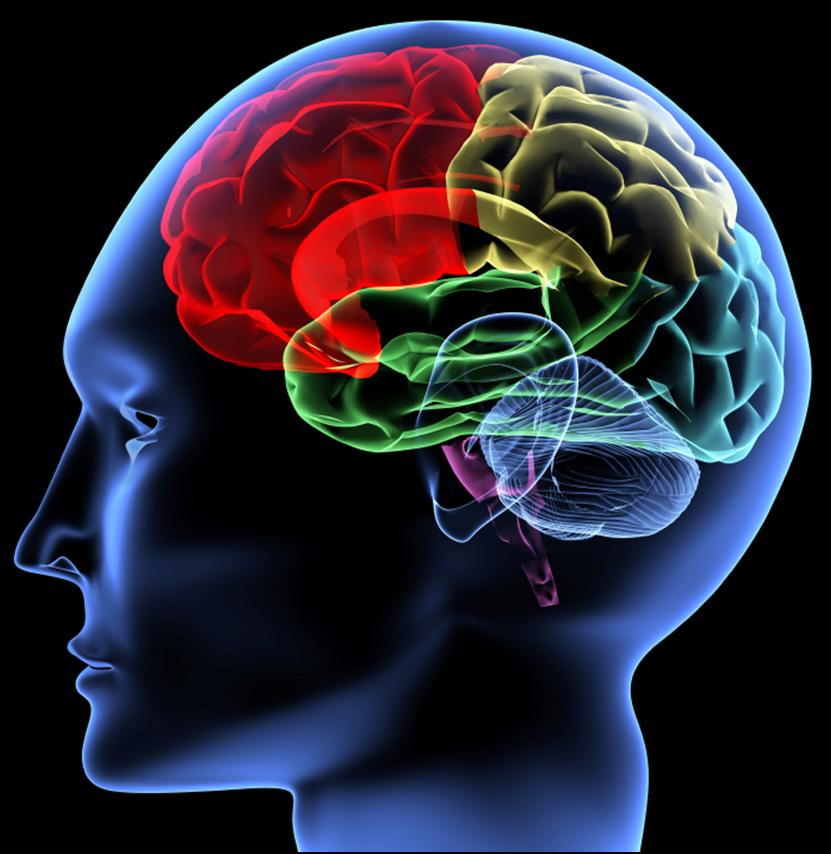
\includegraphics[scale=0.4]{mastermind}
\\\vspace{0.3in}

\includegraphics[scale=0.2]{logHaskell}
\end{center}


%------------------------------------------------------------------------------------------%
\newpage
\subsection{Experiencias}
En realidad fue complicado para todos, el modo de programar en Haskell es totalmente diferente a todo lo que hemos visto anteriormente.\\ Intentamos avanzar el proyecto, pero cada vez que avanzabamos encontrabamos alguna dificultad y nos regresaba de donde hab\'iamos partido, porque as\'i mismo es el lenguaje, funcional y buscando soluciones recursivas.\\
\subsubsection{Experiencias Personales}
No pude entender bien acerca de Haskell, la forma de pensar para prgramar era muy diferente a los otros lenguajes e incluso a los cursos previos que hemos tenido de programaci\'on, esto oblig\'o a poner mayor \'enfasis a la lectura acerca del lenguaje, a\'un as\'i creo que la mayor dificultad estaba en que para trabajar, hab\'ia que usar otro tipo de pensamiento, mas o menos como usar recursividad en funciones que ya eran recursivas y as\'i llamando de un lado a una y otra funci\'on.


\end{flushleft}
\end{document}